%=========================================================================
% (c) Michal Bidlo, Bohuslav Křena, 2008


% xormos00 
% @TODO Radarova rovnica
%       Doplerov Jav?
%       Navrh zaver
%       Vystrignut vsetko pred obsahom a za literaturou, upravit hlavicku
%       Skontroluj literaturu


%Prostudujte dostupnou literaturu týkající se Dopplerova radaru, metod sledování paprsku a způsobů frekvenční analýzy.
%Seznamte se s principy funkce radarů a s principy šíření vyslaného signálu.

% Mind time
%   Zanedbame to, ze sa body na objekte kryju, to spomen
%
%
% Free hustle time
%   Spracuj obrazky


% Teoria
%   Popis interpolaciu?
%   Niquistov teorem

% Uvod
%   Na koniec ked bude vsetko hotove
% Zaver
%   Detto na konci ked bude vsetko hotove
% Teoria
%   Az po praktickej casti popis to co vysvetlujes v praktickej
% Jadro
%
% Poriadne pooznacuj equations
% Skontroluj citacie

\chapter{Úvod}
  \hspace{0.6cm}Táto bakalárska správa predstavuje bakalársku prácu \\\verb|Simulátor širenia radarového signálu|.
  Vznikla za účelom vytvorenia systému pre simulovanie pohybu objektu pred radarom, ktorý predstavuje bežne používaný typ radaru výzkumnou skupinou Fakulty Informačných Technológií v Brne. S pomocou tohto systému by si mali pracovníci výzkumnej skupiny uľahčiť prácu pri testovaní rôznych setup-ov. Pre simulovanie rôznych pohybov, resp. rôznych orientácií voči smeru pohybu. Malo by im to zrýchliť prototypovanie a odhad parametrov aplikácií. Všetky tieto spomenuté úkony sú fizycky a časovo náročné, preto je simulačné riešenie vhodné. 

  Odvetvie radarov je vo svete veľmi rozsiahlo preskumaný a dôkladne popisaný problém, pričom jeho počiatky siahajú do začiatkov 20. storočia a ich najväčší rozvoj nastal v medzivojnovým období hlavne v spojení s leteckým a námorným priemyslom.   
  Ich využitie môžeme v dnešnej dobe vidieť vo viacerých civilných odvetviach vďaka ich priateľným cenovým riešeniam.

  Začiatok tejto práce objasňuje princípy fungovania radaru ako celku, pričom je jeho činosť rozčlenená a vysvetlená do detailov, na úrovni jeho jednotlivých častí. Ďalej je vysvetlené delenie radarov podľa rôznych kritérií a predstavený referenčný radar K-MC4. Neoddelitelnou časťou radaru je pochopenie Dopplerovho javu a Radarovej rovnice. Téma rozoberá šírenie radarového signálu pre ktoré budeme potrebovať pochopiť ako sa paprsky, elektromagnetické vlny radaru šíria priestorom.

  Nasledujúca kapitola predstavuje spôsob spracovania signálu, ktorý sme z radaru získali. Pre získanie požadovaných výsledok musíme najprv z analogového sígnalu vytvoriť digitálny pomocou A/D prevodníku spolu so vzorkovaním a kvantovaním. Zo signálu potrebujeme ďalej odstrániť jednosmernú zložku pre lepšie výsledky a signál nasegmentovať. Okenná funkcia nám signál rozdelí na lepšie spracovatelné časti a po zväčšení frekvenčného rozlíšenia sa môžme pustiť do frekvenčnej analýzy pomocou fourierovej transformácie.

  Názov tejto práce napovedá, že sa jedná o simulátor, k čomu budeme potrebovať základné znalosti o vytváraní modelu a jeho následnej simulácií v porovnaní s referenčným modelom(reálnym radarom)

\chapter{Teoretická časť}
  \section{Radar}
    \hspace{0.6cm}Radar (skratka anglického slova \textbf{RA}dio \textbf{D}irection \textbf{A}nd \textbf{R}anging) je elektromagnetický senzor pre detekciu a lokáciu objektov. Jeho všeobecný princíp fungovania môže byť zhrnutý v  nasledujúcich bodoch\cite{radartutor}\cite{radarhandbook}:
  \begin{itemize}
  \item Radar vysiela zo svojej antény pomocou vysielača elektromagnetické vlny, ktoré sa šíria priestorom v určitom smere.
  \item Niektoré z vysielaných vĺn su zachytené objektmi, ktoré tento signál z jednej časti pohlcujú a súčasne aj odrážajú. Nazývame ich ciele radaru a väčšinou sú v určitej vzdialenosti od radaru, do ktorej má dosah.
  \item Časť tejto energie, ktorá nie je pohltená cieľovým objektom je odrazená naspäť mnohými smermi.
  \item Niektoré vlny z tejto odrazenej, vysielanej energie sa vrátia naspäť k radaru a sú zachytené radarovým príjmačom umiestneným na anténe.
  \item Po zachytení signálu, sú tieto dáta vhodne spracované a analyzované. Vo výsledku zistíme, či su získané informácie naozaj požadované dáta z odrazeného cieľového objektu, ktoré sme chceli vidieť. Alebo len rôzne interferencie prostredia.
  \end{itemize}

  \begin{figure}[h]
      \centering
      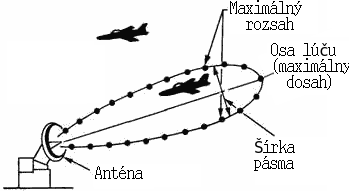
\includegraphics[width=.6\textwidth]{obrazky-figures/radarsk.png}
      \caption{Ukážka funkčnosti radaru \cite{radarimage}.}
      \label{fig:radar}
  \end{figure}

  \subsection{Delenie radarov}
    \hspace{0.6cm}Radary sa delia podľa rôznych kritérií, ako spôsobu tvorby vysielanej energie, typu vysielača a príjmača, či vlnovej dĺžky, atd.

    Základné delenie radarov na \textbf{monostatické} a \textbf{bistatické} určuje či je príjmač a vysielač umiestnený na spoločnej anténe (monostatické), alebo na odelených anténach (bistatické). Bistatickým radarom to umožňuje mať príjmač a vysielač umiestnený na rôzných miestach v priestore, ľubovolne od seba vzdialených\cite{radarsystems}\cite{radarsystem}.

    Dalšie možné delenie radarov je na \textbf{pasívné} a \textbf{aktívne}. Pasívne radary sú tie, ktoré nevysielajú žiadny signál, ale len ho príjmajú. Na jeho základe si utvárajú informácie o okolí. Naproti tomu radary aktívne sa plne podieľajú na vysielaní aj príjmaní signálu.

    Delenie radarov podľa režimu vysielania elektromagnetických vĺn, je to, ktoré bude kľučové pre pochopenie významu tejto práce\cite{radarhandbook}:
    \begin{enumerate}
      \item \textbf{Pulzný radar:} Pracuje len s jednou anténou, ktorá sa nepretržite prepína medzi príjmacím a vysielacím režimom. Vvysiela série elektromagnetických signálov s veľkým výkonom v opakovaných intervaloch. Anténa na krátku dobu vysiela rádio-frekvenčnú energiu rýchlosťou svetla, po prepnutí do príjmacieho režimu čaká na prijatie odrazeného signálu a časový interval medzi vyslaním a prijatím signálu je následne spracovaný. Hlavné využitie pulzného radaru je na veľké vzdialenosti. Jeho najväčší užitok je v oblasti armády. Ostatne je vhodný aj pre aplikácie v riadení leteckej dopravy, predpovedi počasia (obzvlášt pre predpovede zrážok) a v neposlednom rade aj ako radar umiestený na vesmírnom satelite pre vzdialené snímanie povrchu zeme.
      \item \textbf{Radary s kontinuálnou vlnou:} Označované ako CW Radar (\textbf{C}ontinuos \textbf{W}ave Radar) využívajú princíp vysielania kontinuálnej vlny, ktorá je nepretržite vysielaná a príjmaná. Preto CW radar musí obsahovať na svojej anténe dve odelené časti, jednu vysielaciu a druhú príjmaciu. Prenáša signál s konštantnou frekvenciou a amplitúdou. Z dôvodu nemožnosti zmerať čas medzi vyslaním signálu a jeho prijatím nie sme schopný určovať vzdialenosť k objektu. Čo pri pulznom radare nie je problém kedže vieme dobu medzi vyslaním a prijatím signálu, zatiaľ čo u CW radaru nám to nie je známe. Avšak môžme určiť rýchlosť pohybujúceho sa objektu s použitím Dopplerova javu. 

      Rovnako na rozdiel od pulzného radar, CW radar predstavuje v súčasnosti veľmi kompaktné a lacné riešenie pre detekciu objektov. Ktoré sa aplikuje pomocou vstavaných zariadení. Preto v dnešnej dobre zažívajú veľký úspech a nachádzajú využitie v mnohých odvetviach ako napríklad riešeniach v doprave.
    \end{enumerate}
    Radar s kontinuálnom vlnou si v tejto práci určíme ako referenčný.
    Radar K-MC4 od Švajčiarskej spoločnosti RFBeam Microwave GmBH je pre nás implicitný radar a budeme to v tejto práci simulovať. Je to aktívny bistatický radar. Označovaný ako FM-CW radar. \textbf{F}requency-\textbf{M}odulated \textbf{C}ontinuous-\textbf{W}ave. Frekvečne modulovaný radar s kontinuálnom vlnou.

  \subsection{Základne časti radaru}
    \begin{figure}[h]
        \centering
        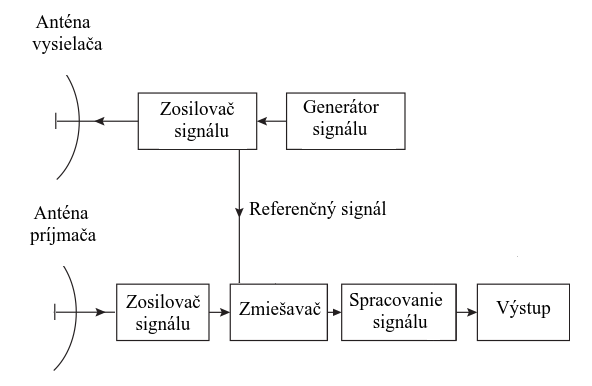
\includegraphics[width=1.0\textwidth]{obrazky-figures/popis_radaru_own.png}
        \caption{Blokové schéme FM radaru.}
        \label{fig:popis_radaru}
    \end{figure}

    Popísané na obrázku \ref{fig:popis_radaru}.
    \begin{enumerate}
      \item \textbf{Anténa (anglicky Antenna):} Je to čo spája radar s vonkajším svetom. Vykonáva viac funkcií: \begin{itemize}
          \item Dovoľuje šíriť vysielanú energiu z vysielača.
          \item Zhromažduje zachytenú energiu odrazenú z cieľa pre príjmač.
          \item Poskytuje informáciu o azimute a elevácii radaru k cieľu.
          \item Jej tvar a veľkosť určujú objem priestoru aký môže radar pokryť
        \end{itemize}
      \item \textbf{Vysielač (anglicky Transmitter):} Dôležitá časť radaru, ktorá generuje a vysiela signál v požadovanej vlnovej dĺžke, Signál je generovaný zo zdroja(\textbf{Generátor signálu}), potrebný výkon sa získava použitím výkonneho oscilátora alebo zosilňovača(\textbf{Zosilovač signálu}(anglicky Amplifier)) spolu s nízkonapäťovým zdrojom.    
      \item \textbf{Príjmač (anglicky Receiver):} Zachytavá a príjma odrazenú energiu z cieľa. Vzhľadom na vzdialenosť a materiál objektu, z akého je zhotovený, sa bude odvíjať jeho intenzita, ktorá dosahuje veľmi malé hodnoty (väčšinou až $10^{-9}$ W). Preto sa signál musí zosíliť pomocou \textbf{Zosilovača}. Pre dalšie spracovanie a je doležité aby anténa neobsahovala žiaden šum, ktorý by mohol skresliť výsledok.
      
      Nasleduje porovnanie prijatého signálu s referenčný signálom, ktorý bol vysielaný. Potom sa môže začať časť spracovania a extrakcie informácii zo signálu. Pomocou rôznych filtrov pre spracovanie signálov.
      %\item \textbf{Prepínač (anglicky Duplexer)} Prvok slúžiaci k tomu aby sa prepínala funkcia prepínača a vysielača na anténe. Touto zmenou funkcie chráni citlivé zariadenie príjmača popritom ako vysielač vysiela. Rovnako presmerúva šum vysielača do príjmača, ktorý ho môže dopredu vyfiltrovať.
      \item \textbf{Zosilňovač (anglicky Duplexer)} V prípade vysielania signálu je jeho úlohou zosíliť signál pred vyslaním, aby sa napriek jeho diaľke, ktorú musí k cieľu uraziť vrátil čo najintenzívnejší. V prípade príjmania signálu ho taktiež zosilňuje, pretože vracajúci sa signál ja veľmi malý.    
    \end{enumerate}

  \section{Charakteristika modulu K-MC4}

    V dnešnej dobre existuje veľké množstvo výrobcov radarov, ktoré ich produkujú v rôznych tvaroch a typoch. S rôznymi charakteristikami a možnosťami. Pre túto prácu si zvolíme modul K-MC4 predstavujúci radar, ktorého činosť budeme v simulovať. Zvolili sme ho hlavne z dôvodu jeho častého využitia vedeckou skupinou zaoberajúcou sa radarmi na Fakulte Informačných Technológií, Vysokého Učení Technického v Brne.

    \begin{figure}[h!]
        \centering
        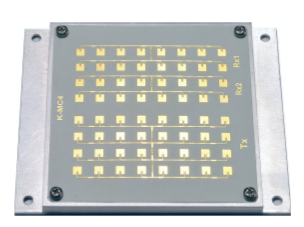
\includegraphics[width=.4\textwidth]{obrazky-figures/kmc4fyz.png}
        \caption{Radar K-MC4 od Švajčiarskej spoločnosti RFBeam Microwave GmBH \cite{kmc4sheet}}
        \label{fig:kmc4fyz}
    \end{figure}

    \subsection{Základné vlastnosti radarového modulu\cite{kmc4sheet}:}
    \begin{itemize}
      \item 24 GHz vysielacia frekvencia, pomocou nízko-dosahového monopulzného vysielača
      \item Dvojitý príjmač s +/- 15$^{\circ}$ pokrytím
      \item Rozptyl vysielaného lúču 30$^{\circ}$/ 12$^{\circ}$ @ -3dB
      \item 180MHz FM(Frekvenčná modulácia) - vstup
      \item Integrovaný vysoko citlivý RF/IF(intermediate
frequency) zosilovač
      \item I/Q IF výstup z oboch kanálov
      %\item Temperature compensated oscillator
      \item Technika rýchleho prebudenia šetriaca enerigiu RSW (Rapid Sleep Wakeup).
      \item Extrémna kompaktnosť 78x98x7mm
    \end{itemize}

    \begin{figure}[h!]
        \centering
        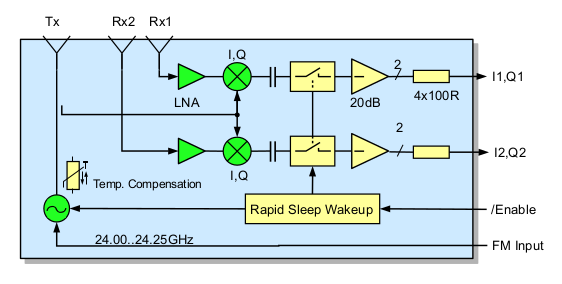
\includegraphics[width=1.0\textwidth]{obrazky-figures/radar_kmc4.png}
        \caption{Blokové schéma radaru K-MC4 \cite{kmc4sheet}}
        \label{fig:radar_kmc4}
    \end{figure}

    K-MC4 je Dopplerov radar s asymetrickým vysielačom a dvoma prijmacými antenámi. Ktoré lepšie napomáhajú k vyhodnoteniu rýchlosti meraného objektu. Ten svojím pohybom k radaru mení uhol snímania a signál postupne zaostáva. Táto technika je často nazývaná \verb|monopulzný radar|, čo je vlastne \verb|fázové porovnávanie signálu|. Vysielacia odchýlka +/- 15$^{\circ}$ od hlavnej osi spôsobuje odchýlku +/-100$^{\circ}$ v cieli. So zvyšujúcim sa uhlom sa znižuje prenosť nameraných hodnôt.

    Funkciu týchto dvoch príjmacích a jednej vysielacej antény v našej simulácii zahrnieme, pretože nám to pomože určiť orientáciu objektu voči radaru(znázornené na obrázku \ref{fig:kmc4_odchylka}). To znamená v akom smere sa objekt pohybuje. Od resp. k radaru alebo či prechádza pred radarom z ľavej strany smerom do pravej alebo z pravej strany smerom do ľavej.   

    Pohybujúci sa objekt generuje Dopplerov signál na oboch kanáloch I a Q (znázornené na schéme obrázku \ref{fig:radar_kmc4}). Fázový posun medzi Ix a Qx indikuje smer pohybu objektu. Približujúci sa objekt generuje 90$^{\circ}$ medzi výstupmi I a Q, vzdiaľujúcii sa objekt generuje naopak -90$^{\circ}$.

    Funkcia RSW, technika rýchleho prebudenia je ideálna pre používanie s batériou\cite{kmc4sheet}. To avšak v tejto práci, ktorá je simulačná nepovažujeme za potrebné a túto funkciu zanedbáme.
    \newline

    \textbf{Využitie modulu K-MC4:}
    \begin{itemize}
      \item Určovanie vzdialenosti, smeru a rozmerov objektov.
      \item Zisťovanie rýchlosti objektov.
      \item Industriálne senzory.
    \end{itemize}


    \begin{figure}[h!]
        \centering
        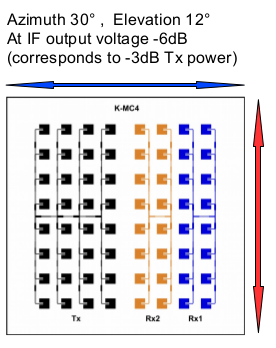
\includegraphics[width=.45\textwidth]{obrazky-figures/kmc4_odchylka.png}
        \caption{Obrázok ilustrujúci anténu radaru KMC-4. Štvorčeky označené čaiernou farbou reprezentuju vysielač ($Tx$) radaru. Žltou ($Rx2$) a modrou ($Rx1$) farbou sú znazornené obe príjmače. Povrch jedného príjmača je polovica z povrchu vysielača. 
        Červená šipka reprezentuje horizontálnu a modrá vertikálnu osu radaru, ktorá je potrebná pre výpočet straty signálu.\cite{kmc4sheet}.}
        \label{fig:kmc4_odchylka}
    \end{figure}

  \section{Doplerov jav}
  \hspace{0.6cm}Doplerov efekt popisuje zmenu vlnovej dlžky príjmaného signálu voči signálu vysielanému. Čo je spôsobené nenulovou vzájomnou rýchlosťou prímača a vysielača.
  Tento jav nenastáva len pri zvuku, no obecne je pozorovateľný pre ľubovolné elektromagnetické vlnenie. 
  Vlnová dĺžka vysielaná z vlnového zdroja(zvuku, elektromagnetického žiarenia, svetla, atd.) narazí na pohybujúci sa objekt. V závislosti na smere pohybu tohto objektu, sa vlnové dĺžky "stlačia", alebo "rozťiahnu", čo vo výsledku vedie k zmene frekvencie. Odrazený signál so zmenenou frekvenciou sa napríklad pri zvuku prejavý zmeneným tónom pre poslucháča. Teda zmiešaním frekvencie je vo výsledku zmena prechodovej sínusovej frekvencie. Nezáleží či sa pozorovateľ pohybuje k zdroju alebo zdroj k pozorovateľovi\cite{radarsensing}\cite{radarsystems}.
  
  Dopplerova frekvencia sa dá vypočítať ako dvojnásobok rozdielu frekvencií ($2 f_{0}$) násobený podielom rýchlosti vozidla ($v$) k rychlosti svetla ($c_{0}$) a kosínusom uhlu pohybu objektu k pozorovateľovi ($\cos \alpha$), znázornené v rovnici \ref{eq:0}.

    \begin{equation} \label{eq:0}
      f_{Dopp} = 2 f_{0} \frac{v}{c_{0}}\cos \alpha
    \end{equation}
        

  \section{Radarová rovnica} \label{radarovarovnica}

    Jedna zo základných rovníc radarovej teórie je radarová rovnica. Ktorá nám z pomedzi iného slúži nielen na zistenie dosahu radaru, ale rovnako ako aj ako charakteristika radarového systému. Radarová rovnica pre vojenské radary je jemne rozdielna od tej pre konvenčné radary, alebo iné typy radarov. Každá jedinečná aplikácia radaru vo všeobecnosti potrebuje využiť radarovú rovnicu upravenú k daným špecifikáciam, požiadavkám a aplikáciám. Napríklad podľa použitia radaru v rôznom prostredí a to na zemi, vo vzduchu alebo vo vode.

    Anténa služi na usmernenie vyžarovaného energie v správnom smere. Rovnica energie prijatého signálu je definovaná ako súčinu vysielanej energie [$W$], a zisku anténý ($G$):
    \begin{equation} %\label{eq:0}
      P_{d} = \frac{P_{t} * G}{4\pi * R^{2}}
    \end{equation}

    Zisk antény G je definovaný ako súčin zisku vysielača ($Ft$) a príjmača ($Fr$):
    \begin{equation} %\label{eq:0}
      P_{d} = \frac{P_{t} * F_{r} * F_{t}}{4\pi * R^{2}}
    \end{equation}

    \hspace{0.6cm}Vyslaná energia ktorá dopadá na objekt je pohltená alebo rozptýlená do prostredia, avšak malá časť sa odrazí a vracia k radaru. Jedná sa o veľmi malú časť oproti veľkosti vyslaného signálu. Objekty podľa svojho tvaru, materiálu a povrchu odrážajú naspäť rôzne množstvo energie. Táto hodnota je vyjadrená ako $RCS$ (\textbf{R}adar \textbf{C}ross-\textbf{S}ection), odrazivej plochy radaru. Hodnota $RCS$ sa vyjadruhe v $m^{2}$.
    
    Vzdialenosť objektu sa počíta ako súčin vzdialenosti príjmača radaru od objektu a vysielača radaru od objektu. V našom prípade je vysielač aj príjmač umiestnený na jednej anténe a budeme ho označovať ako $d^{2}$.
    
    Hodnota $loss$, rezprezentuje stratu signálu vzhľadom na uhol, pre ktorý je pravý uhol bod, na ktorý radar priamo miery.

    Výsledná radarová rovnica, ktorá obsahuje všetky potrebné hodnoty pre náš projekt a má tvar:
    \begin{equation} %\label{eq:0}
      P_{r} = \frac{P_{t} * F_{r} * F_{t} * RCS}{(4\pi)^{2} * d^{4} * loss}
    \end{equation}

    \hspace{0.6cm}Dosah radarového paprsku je daný radarovou rovnicou, ktorá pojednáva o maximálnom dosahu vysielaného paprsku tak aby bol znova úspešne prijatý príjmačom. Táto vzdialenosť záleži od výkonu vysielača radaru a úspešnosti šírenia sa vlnenia priestorom.
    %Šírenie radarového lúča v priestore zavysí od mnoho aspektov.

    Index lomu popisuje ako sa elektromagnetické žiarenie z radaru šíri a láme v rôznom prostredí\cite{radarbeam}.
        
\section{Spracovanie signálu}
    \hspace{0.6cm}Výstup radaru je reprezentovaný analógovým signálom, ktorý odpovedá frekvencii generovanej pohybujucím sa objektom pred radarom. Cieľom spracovania signálu je prevedenie frekvenčnej analýzy, ktorej výstupom sú užitočné informácie o objekte ako napríklad jeho rýchlosť a vzdialenosť.

    Pred samotnou frekvenčnou analýzou a úpravou signálu je potreba ho zdigitalizovať pomocou A/D prevodníku. Proces prevodu signálu z analógovej podoby do digitálnej pozostáva z dvoch procesov a to Vzorkovania a Kvantovania\cite{radarsystemproc}.\newline

  \subsection{Vzorkovanie a Kvantovanie}

    \hspace{0.6cm}Vzorkovaním rozumieme násobenie pôvodného signálu sledom periodických obdlžníkových signálov nenulovej šírky (tzv. Dirakových impulzov). Je potrebné tieto impulzy navrhnúť tak, aby nevzniklo skreslenie spôsobené nami volenou šírkou obdlžníka.
    Násobenie signálu v čase odpovedá konvolúcii ich spektier, čo je postupnosť kópií spektra pôvodného signálu s periodou vzorkovacej frekvencie, rovnica \ref{eq:2}\cite{issslajdy}.

    \begin{equation} \label{eq:2}
      F_{S} = \frac{1}{T}
    \end{equation}

    Ak bude vzorkovacia frekvencia príliš nízka, budú sa jednotlivé kópie pôvodného spektra prekrývať. V takom prípade nebudeme môcť navzorkovaný signál rekonštruovať späť do pôvodnej podoby. To sa označuje ako antiliasing. Aby sme tomu zabránili musíme dodržať Nyquistov-Shannonov vzorkovací teorém, znázornený vo vzťahu \ref{eq:3}. Maximálna frekvencia signálu musí byť nižšia než polovica vzorkovaciej frekvencie.

    \begin{equation} \label{eq:3}
      F_{S} > 2 f_{max}
    \end{equation}

    % \hspace{0.6cm}Kvantovanie je diskretizácia oboru hodnôt signálu, pričom je tento proces stratový a nezvratný. Podstatou jeho činnosti je zaokrúhlenie hodnôt navzorkovaného sginálu na predom definované kvantizačné hladiny. Najdoležitejšie je správne nastavenie kvantizačnej hladiny, to je poväčšine priamo závislé na citlivosti snímaneho zariadenia.\cite{issslajdy}\newline
    Kvantovanie prevedie rozsah signálu na diskretny signál. Kvantizovaný signál vezme len diskrétne, zvyčajne konečné súbory hodnôt. Narozdiel od vzorkovania, kde pomocou vhodných podmienok je možná presná rekonštrukcia signálu, kvantizácia je nezvratný proces a vo výsledku je možná stráta informácií. Podstatou jeho činnosti je zaokrúhlenie hodnôt navzorkovaného sginálu na predom definované kvantizačné hladiny.\cite{issslajdy}\newline 

    \begin{figure}[h]
        \centering
        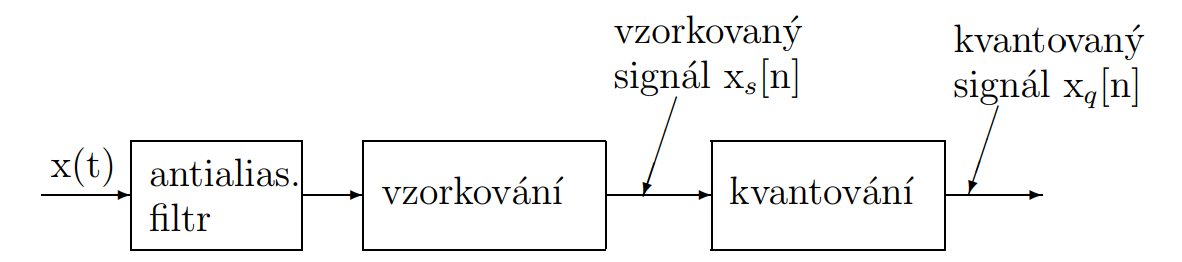
\includegraphics[width=.9\textwidth]{obrazky-figures/adprevod.png}
        \caption{Diagram odchýlky vysielania antény \cite{zreopora}.}
        \label{fig:adprevod}
    \end{figure}

  \subsection{Odstránenie jednonosmernej zložky}

    \hspace{0.6cm}Po digitalizácii singálu odstránime jednosmernú zložku, ktorá je vyjadrená ako stredná hodnota signálu. Tú môžeme vypočítať priemerovaním singálu, rovnica \ref{eq:4}. 

    \begin{equation} \label{eq:4}
      \bar{s} = \frac{1}{N} \sum_{n=1}^{N} s[n]
    \end{equation}
    %s s ciatkou = 1 lomeno N Sigma n=1  nad N s[n]

    Ak sa blíži k nule, tak sa v signále jednosmerná zložka nevyskytuje. Naopak ak je rôzna od nuly, tak v signále nenesie žiadnu užitočnú informáciu, práve naopak nám môže pri dalších výpočtoch zastrieť požadované informácie v signále. Jej odstránenie prevedieme práve odčítaním tejto strednej hodnoty.\cite{zreopora}\newline

  \subsection{Segmentácia}

    \hspace{0.6cm}Segmentácia je delenie signálu na menšie časti - rámce. Rámce su úseky signálu, vzniknuté z pôvodného signálu. Toto rozdelenie potrebujeme pre dalšie zpracovanie.
    Dlžka rámcov by mala byť dostatočne malá nato, aby bolo možné pokladať signál na danom úseku za stacionárny. Avšak rovnako by mala byť taká veľká, aby sme mohli čo najpresnejšie odhadnúť požadované parametry signálu.
    Veľkosť rámca sa často volí ako mocnina čislice dva ($2^{1}, 2^{2}, ... , 2^{n}$). Čím rýchlejšie sa bude objekt pohybovať, tým väčšiu veľkosť rámca zvolíme\cite{zreopora}.

    \hspace{0.6cm}Okenná funkcia minimalizuje rozptyl tvarovaním hondôt signálu v segmente, ktorý spôsobuje Fourierova transformácia použitá na neperiodický signál.
    Existuje mnoho okenných funkcií, ktoré môžme aplikovať v zavíslosti na tom aký je požadovaný signál. Každá mení výsledok spektra trochu iným spôsobom. 
    Výber správnej okennej funkcie nie je jednoduchá úloha. Každé okno má svojú vlastnú charakteristiku a vhodnosť pre rôzne druhy signálov. Dôležite je avšak zvoliť vhodnú okennú funkciu na daný typ dát.

    Dve najefektívnejšie okenné funkcie pre použitie v radaroch sú \verb|Hammingovo okno| a \verb|Hanningovo okno (Hann)|. Obe sú reprezentované sinuusovým tvarom. Obe pripomínajú tvar kopca. Avšak, Hanningovo okno sa dotýka nuly na oboch koncoch a tým zabezpečuje kontinuitu signálu. Hammingovo okno nedosahuje na okrajoch presnej hodnoty nula a preto stále obsahuje určitú diskontinuitu signálu. Tieto okenné funkcie sú vhodné pre meranie šumu signálu a majú lepšiu frekvenčné rozlíšenie ako iné okenné funkcie a popritom zachovávajú dobrú presnosť.\cite{radarmatlab}\cite{undestandingfft}\newline

    \begin{figure}[h]
        \centering
        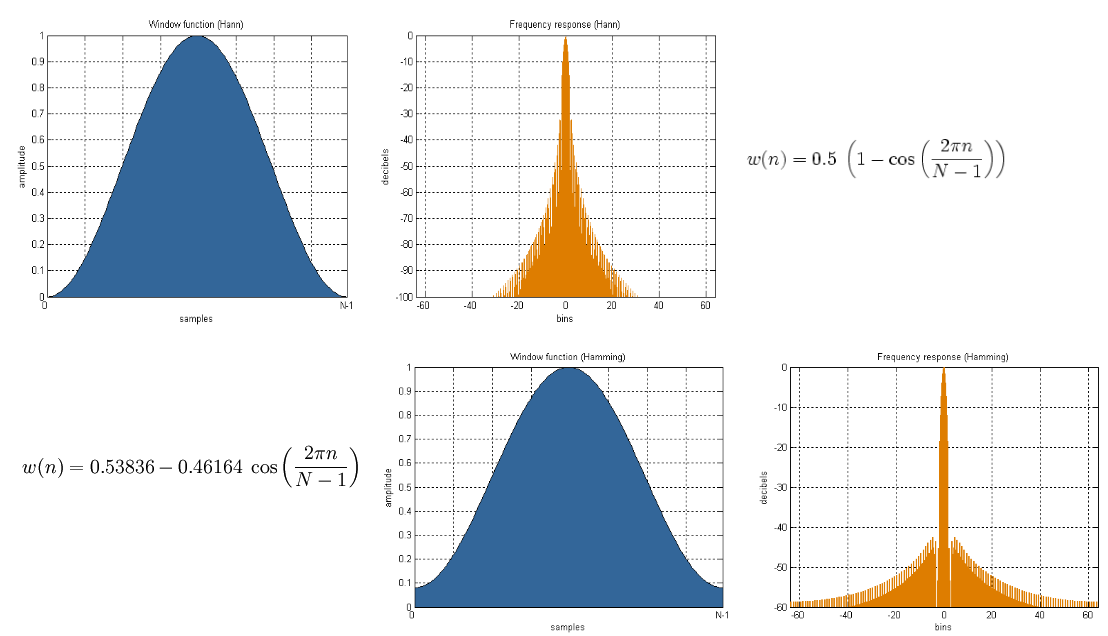
\includegraphics[width=.9\textwidth]{obrazky-figures/okennefunkcie.png}
        \caption{Okenná funkcia Hanning (hore) a okenná funkcia Hamming (dole) a ich frekvenčná odozva pre funkciu sínus\cite{flexradio}.}
        \label{fig:okennefunkcie}
    \end{figure}

  \subsection{Zero-padding}

    \hspace{0.6cm}Frekvenčné rozlíšenia záleží na počte spracovaných vzorkov. Ak sa teda do analyzovaného signálu pridajú vzorky, v našom prípade metódy \verb|zero padding| nuly, zvýšime tým vo výsledku frekvenčné rozlíšenie spektra.
    Dôvod prečo chceme mať na konci vzorku nuly je aby vzorka signálu mala hodnoty mocniny dvojky. Ak je časové spektrum signálu reprezentované mocninou dvojky, zvýší to rýchlosť spracovania signálu Rýchlou Fourierovou Transformáciou, ktoru si vysvetlíme v dalšej časti.
    Dôležité si je uvedomiť, že touto metódou nepridávame do spektra žiadnu novú informáciu.\cite{understandingsignals}\newline


  \subsection{Frekvenčná analýza}

    \hspace{0.6cm}Signál máme reprezentovaný v časovom spektre, pre jeho dalšie spracovanie a získanie potrebných informácií ho potrebujeme previesť do frekvenčného spektra. Tým, jednoducho povedané, dostaneme rovnaký signál s iným vzhľadom. Najlepšie nám na to poslúži matematická funkcia - Diskrétna Fourierova transformácia (DFT). Nami používaná metóda bude Rýchla Fourierová transformácia (FFT), ktorá je lepšie optimalizovaná a rýchlešia metóda ktorá vznikla z DFT, vykazujúca rovnako dobré výsledky ako DFT. Jej funkčnosť v jednoduchosti znamená, že zoberie signál a rozloží ho na sínusové vlny rôznych amplitúd a frekvencií\cite{understandingsignals}\cite{undestandingfft}.\newline

    Diskrétna Fourierova transformácia vznikla z Fourierovej transformácie, od ktorej sa líší tým, že pracuje s dikrétnym časom. DFT definuje sekvenciu diskrétnych hodnôt frekvenčného rozsahu, znázornené v rovnici \ref{225a}.

    \begin{equation} \label{eq:225a}
      F(n) = \sum\limits_{n = 0}^{N-1} f(k) e^{-j2\pi n k / N}  
      (n = 0..1,...,N-1)
    \end{equation}

    $F(n)$ reprezentuje výsledný frekvenčný rozsah. $f(k)$ je diskrétna sekvencia v časovom rozsahu, $k$ reprezentuje index v danom frekvenčnom rozsahu, a $n$ index v danom časovom rozsahu. $N$ predstavuje celkový počet vzoriek. Všetky hodnoty F(n) sú reprezentované prostredníctov reálnej a imaginárnej zložky čísla, ktoré sú znázornéné na obrázku \ref{fig:real_imag}. Budeme ich ďalej v práci označovať ako I a Q. Z týchto dvoch zložiek môžeme zistiť fázový posun a to pomocou podielu imaginárnej a reálnej zložky, ktorá je prevedená cez inverznú trigoniometrickú funkciu tangens. Frekvencia snímkov $F(n)$ je vyjadrená v rovnici: 

    \begin{equation} \label{eq:225b}
      F_{\alpha}(n) = tan^{-1}(\frac{F_{imag}(N)}{F_{real}(N)})
    \end{equation}\newline   

    \begin{figure}[h!]
        \centering
        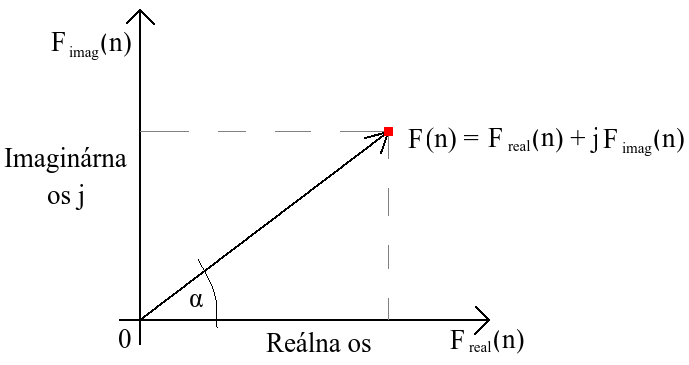
\includegraphics[width=.85\textwidth]{obrazky-figures/real_imag.png}
        \caption{Vzťah komplexnej hodnoty F(n)\cite{undestandingsignals}}
        \label{fig:real_imag}
    \end{figure}
   
  \subsection{Interpolácia}
    %V situácií kedy meráme závislost nejakej fyzikálnej veličiny na čase.
    \hspace{0.6cm} Interpolácia je matematická metóda, ktorá nám služí na nájdenie približnej hodnoty funckie v nejakom intervale, ak je nám jej hodnota známa v iných bodoch tohoto intervalu.
    
    Metóda pozostáva z odhadu hodnôt bodov danej funkcie medzi jej zadanými hodnotami $(x_{0}, y_{0}), (x_{1}, y_{1}), ... (x_{n}, y_{n})$. Hodnoty interpolujeme pre nejaký interval, vždy medzi dvojicou bodov. Do výpočtu nám vstupujú hodnoty z daného intervalu, ktorý počítame, rovnako aj hodnoty z predchádzajúceho a nasledújuceho intervalu. Týmto spôsobom sa dosiahne hladšia a presnejšia interpolácia

    V našej práci použijeme interpoláciu Spline, ktorá oproti iným interpolačným metódam prináša najviac spojité spojenie týchto hodnôt na celom intervaly. Metóda je ilustrovaná na obrázku \ref{fig:spline}. \cite{inmopora}
    \begin{figure}[h!]
        \centering
        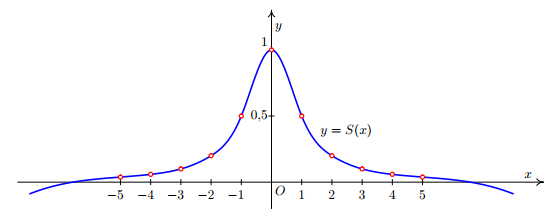
\includegraphics[width=.85\textwidth]{obrazky-figures/spline.png}
        \caption{Grafická ukážka interpolačnej funkcie spline. Ktorá prirodzene spája body\cite{inmopora}.}
        \label{fig:spline}
    \end{figure}        

\section{Modelovanie a simulácia}

  \hspace{0.6cm}\textbf{Simulácia} je metóda získavania nových poznatkov o systéme experimentovaním s jeho modelom. Pre účely simulácie musí byť model popísaný odpovedajúcim spôsobom.

  \textbf{Model} je napodobenina systému iným systémom, napríklad v našom prípade napodobenina reálneho, fyzického radaru počítačovým programom. Model musí pre naše účely napodobňovať všetky podstatné vlastnosti systému.

  \textbf{Systém} môžeme všeobecne definovať ako súbor elementárnych častí, prvkov systému, ktoré majú medzi sebou nejaké väzby, prepojenia.

  \textbf{Modelovanie a simulácia} je proces vytvárania modelu systému na základe našich znalostí získaných o systéme. Kvalita vytvoreného modelu v zásade ovplyvní výsledky získané experimentovaním s modelom.\cite{imsopora}

  \begin{figure}[h!]
      \centering
      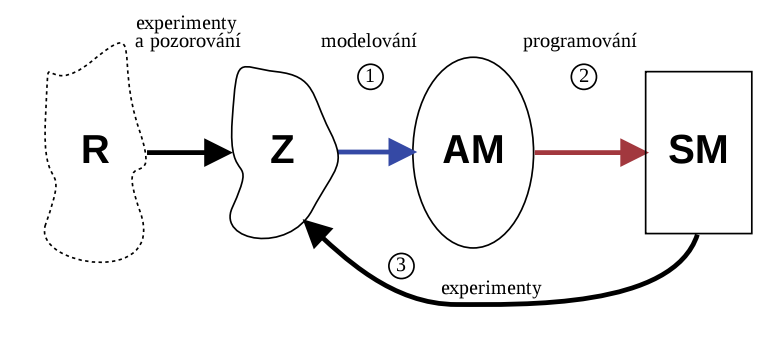
\includegraphics[width=.85\textwidth]{obrazky-figures/simulacia.png}
      \caption{Celý proces modelovania a simulácie  Realita $\rightarrow$ Znalosti $\rightarrow$ Abstraktní Model $\rightarrow$ Simulační Model\cite{imsopora}}
      \label{fig:radar_kmc4}
  \end{figure}

  \subsection{Princípy}
    \begin{enumerate}
      \item Vytvoríme abstraktný model(AM), ktorý zahrňuje naše získané znalosti o systéme, ale zahrňujeme len tie, ktoré su pre naše účely podstatné. Jeho forma môže byť napríklad pomocou matematických rovníc.
      \item Na základe abstraktného modelu vytvoríme simulačný model(SM), ktorý už nezjednodušuje a musí zahrňovať všetky vlastnosti AM. SM je spustitelný program, ktorý počíta výsledky podľa zadaného počiatočného stavu, vstupov a parametrov modelu. V našom prípade sa musí správať ako referenčný radar K-MC4. 
      \item So simulačným modelom vykonávame simulačné experimenty a výsledky analyzujeme.
    \end{enumerate} 

  \subsection{Diskrétny systém a simulácia}
    \hspace{0.6cm}Pod pojmom diskrétny systém rozumieme systém s konečným počtom stavov.
    Diskrétny sýstem je často modelovaný vo forme orientovaných grafov a je pravdivostne analyzovaný pomocou algoritmov. Pretože diskrétne systémy maju daný počet stavov, môžu byť charakterizované aj pomocou presných matematických modelov.

    Počítač je konečný stavový automat, ktorý môže byť vnímaný ako diskrétny systém. Pretože počítače sú často používané pre modelovanie, nie len diskrétnych systémov ale rovnako aj prechodných systémov boli vyvinuté metódy ako reprezentovať prechodné modely reálneho sveta ako diskrétne systémy.

    Jednotlivé, v reálnych systémoch prebiehajuce procesy môžme popísať sekvenciou krokov alebo príkazmi programovacieho jazyka. Takáto postupnosť príkazov vyjadruhe cohvanie celej triedy procesov. Ak máme viac procesov (paralelné procesy) musíme zaistiť ich vzámojnú komunikáciu, napríklad prostredníctvom správ. Súčasťou popisu chovania procesov musí byť taktiež zaistenie ich synchronizácie pri používaní zdieľaných prostredkieov\cite{imsopora}.

  \subsection{Simulovanie činnosti radaru}

    \hspace{0.6cm}Je veľa spôsobov ako popísať diskrétny systém. V tejto práci použijeme popis programom v programovacom jazyku, vo forme procesov.
    Snažíme sa zamerať na simuláciu radaru so zjednodušenou fyzikálnou podstatou problému správneho nasimulovania radaru. To znamená, že sa sústredime hlavne na správnu simuláciu prostredia a šírenia samotného signálu, viac ako na fyzikálnu podstatu širenia tohto signálu. A to napríklad tak, že zanedbáme fyzikálne vlastnosti prostredia v ktorom sa bude šíriť.

\chapter{Návrh}

  \hspace{0.6cm}V tejto kapitole sa budeme venovať návrhu a riešeniu simulácie šírenia radarového signálu. Pomocou získanej a vysvetlenej teoretickej časti prechádzame na kapitolu návrhu, kde si načrtneme nami vytvorené riešenie, ktore v ďalšej implementačnej časti následne použijeme.

  \section{Radar v priestore}
    \hspace{0.6cm}V návrhu simulačného prostredia si pre jednoduchosť vysvetlenia predstavme kocku, ktorá tvorí náš priestor pre umiestnenie radaru, objektu a definovanie podmienok, ktoré pre simuláciu radaru potrebujeme. Ako scénu si predstavme meranie rýchlosti na diaľnici s použitím radaru umiestnenom na vyvýšenou mieste, ktorý sleduje vozidlá na vozovke pod ním.

    V priestore je teda umiestnený radar, pre predstavu napríklad na dialničnom moste, ktorého zorné pole smeruje na diaľnicu pod nim, teda objekty, ktoré radar sleduje ho míňajú po jeho vertikálnej ose, teda prechádzajú pod ním.
    % Táto predstava je základná a postavenia sa budú dať meniť. 

    \begin{figure}[h]
        \centering
        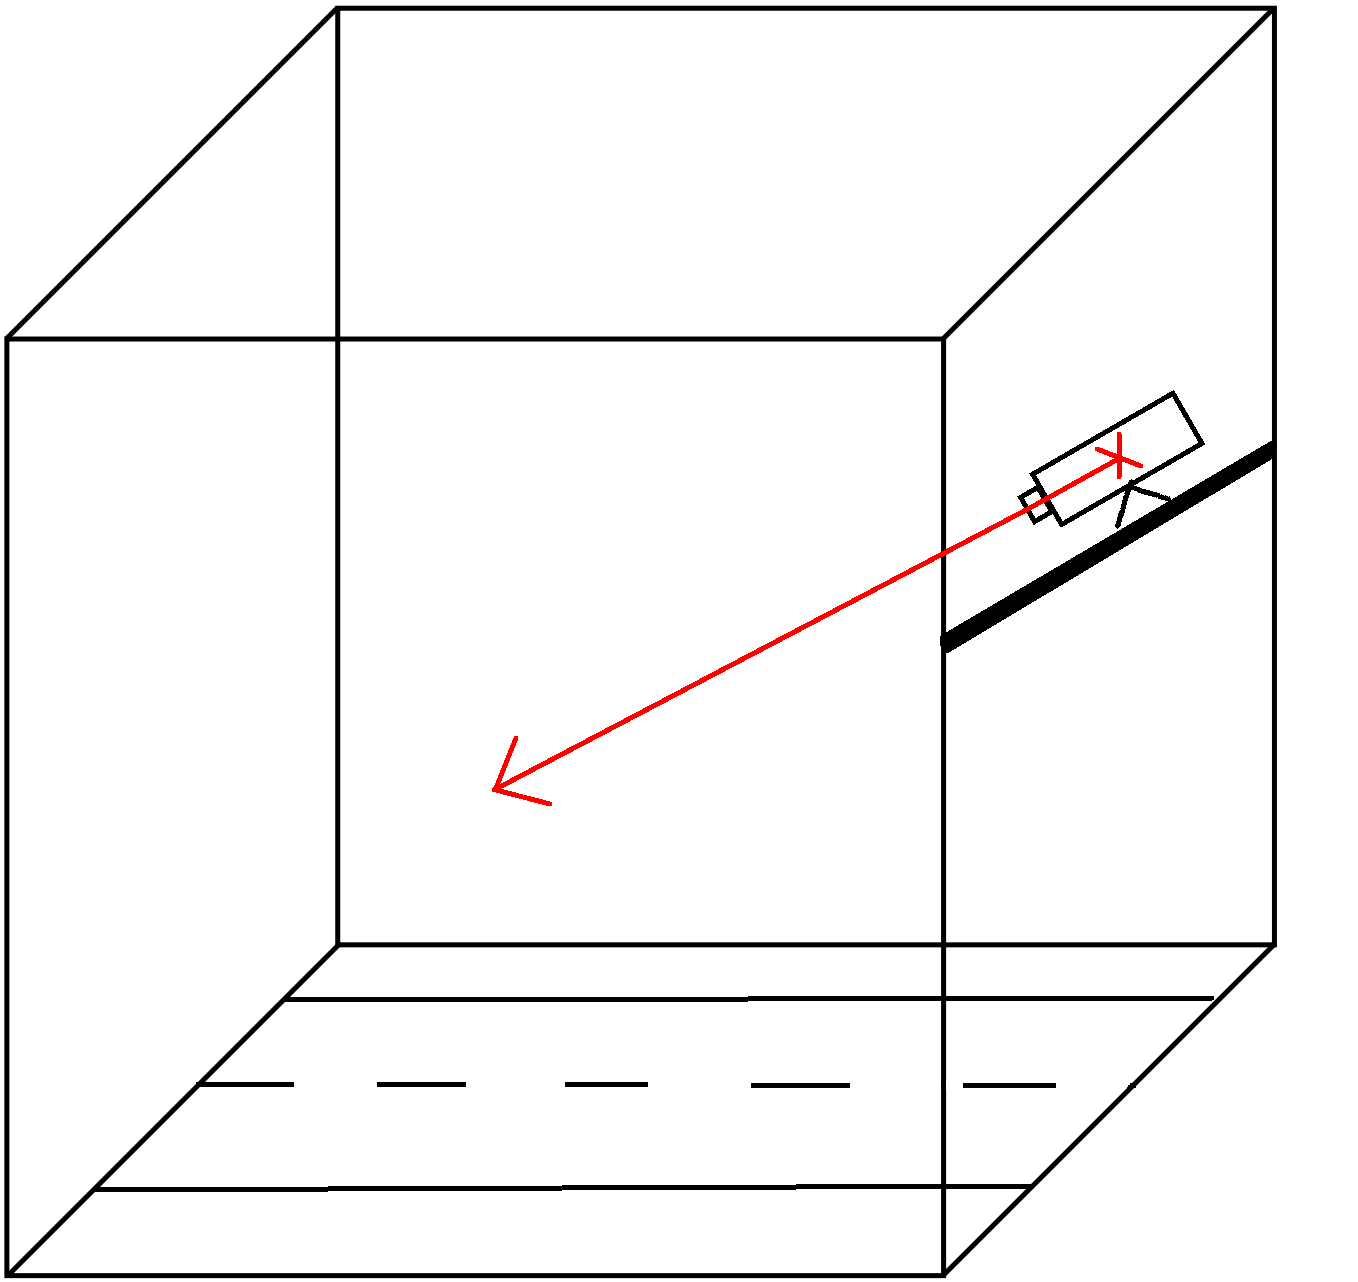
\includegraphics[width=.5\textwidth]{obrazky-figures/cube_radar.png}
        \caption{Základná predstava priesotru, ktorý budeme simulovať.}
        \label{fig:cube_radar}
    \end{figure}

    Radar bude reprezentovaný ako práve jeden nehybný bod v priestore. Tento bod má mať presne určené svoje súradnice v priestore, ktoré charakterizujú jeho polohu. Rovnako obsahuje vektor, ktorý určuje bod, kam radar mieri. To znamená, že je nevyhnutne dôležité vedieť kam radar presne mieri počas celej simulácie. Radar bude možné jednoducho natáčať po vertikálnej a horizontálnej ose pomocou tohto vektoru, znázornené na obrázku \ref{fig:cube_radar}. 
    Dodatočne môžeme pridať aj naklonenie radaru na mieste, do strán. Týmto spôsobom pri naklonení na mieste v 90$^{\circ}$ uhle získame prehodenie jeho vertikálnej a horizontálnej osi.
    ;
    Bod definujúci polohu radaru bude slúžiť ako miesto pre generovanie signálu a zdroj vysielania paprskov na vektor zorného poľa radaru. Podľa súradníc polohy radaru a vektoru radaru sme schopný určiť nevyhnutné uhly a vzdialenosti, ktoré budeme potrebovať pre výpočty simulácie.

  \section{Objekt v priestore}
    \hspace{0.6cm}Pre správnu funkciu radaru a získanie čo najväčšieho množstva simulačných dát je potrebné rovnako ako aj v návrhu samotného radaru, aj čo najpresnejšie popísať objekt na ktorý budeme v simulácii vysielať naše paprsky, teda cieľ radaru. 

    \begin{figure}[h]
        \centering
        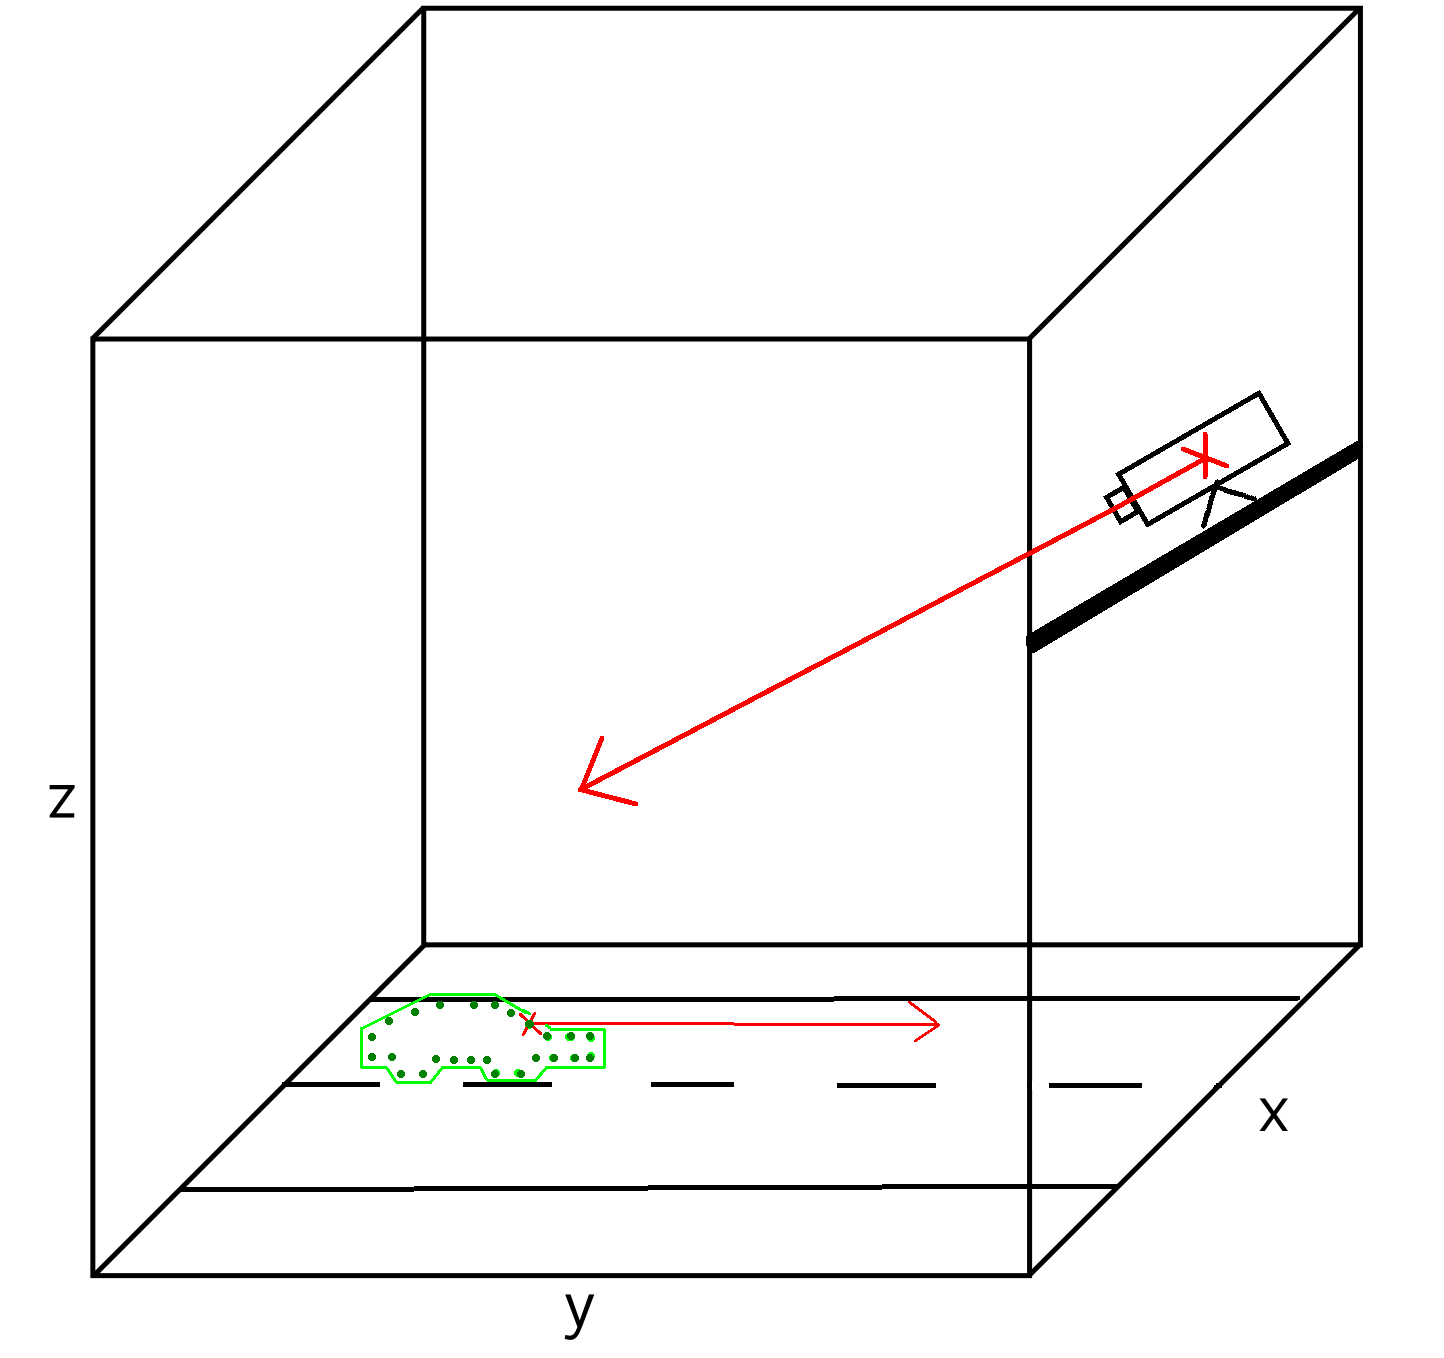
\includegraphics[width=.5\textwidth]{obrazky-figures/cube_radar_car.png}
        \caption{Základná predstava priesotru, obsahujúci cieľový objekt.}
        \label{fig:cube_radar_car}
    \end{figure}    

    Objekt preto budeme reprezentovať ako zhluk bodov v určitom tvare, ktorý pripomína objekt reálneho sveta, ako napriklad v našom návrhu, osobné vozidlo.

    Každý tento bod objektu, pričom počet bodov ohraničujúci objekt bude vopred určený, bude pre radar vnímaný ako samostatný objekt a bude obsahovať svoje súradnice v priestore.
    Každý tento bod, sám o seba taktiež objekt bude vykonávať pohyb v priestore, čo bude reprezentovať pohyb celého objektu. Tento pohyb bude reprezentovaný vektorom pohybu bodu, súradnice objektu môžeme pomocou vektoru pohybu odpovedajúcim spôsobom modifikovať.
    Súčasťou vektoru bude aj rýchlosť pohybu objektu, ktorá bude dopredu definovaná a potrebná pre dalšie výpočty. 
    Všetky body v objekte sa teda budú zdanlivo pohybovať ako jeden celok, znázorne

    Podstatnou charakteristikou bodu bude jeho RCS (Radar Cross-section), ktorý reprezentuje ako intenzívne bude daný bod reagovať na prijatý signál, teda akou silou a smerom odrazi signál näspať. To všetko závisí na simulovanom tvare a materiálu objektu, rovnako ako aj uhlom pod akým je voči paprsku. RCS sa bude dať jednoducho nastaviť ako vstupná hodnota programu. Rovnako ako súradnice umiestnenia bodov, rýchlosť objektu, charakterisitka radarového modulu a nastavenia simulácie.

  %\section{Princíp sledovania paprsku}


    \begin{figure}[h]
        \centering
        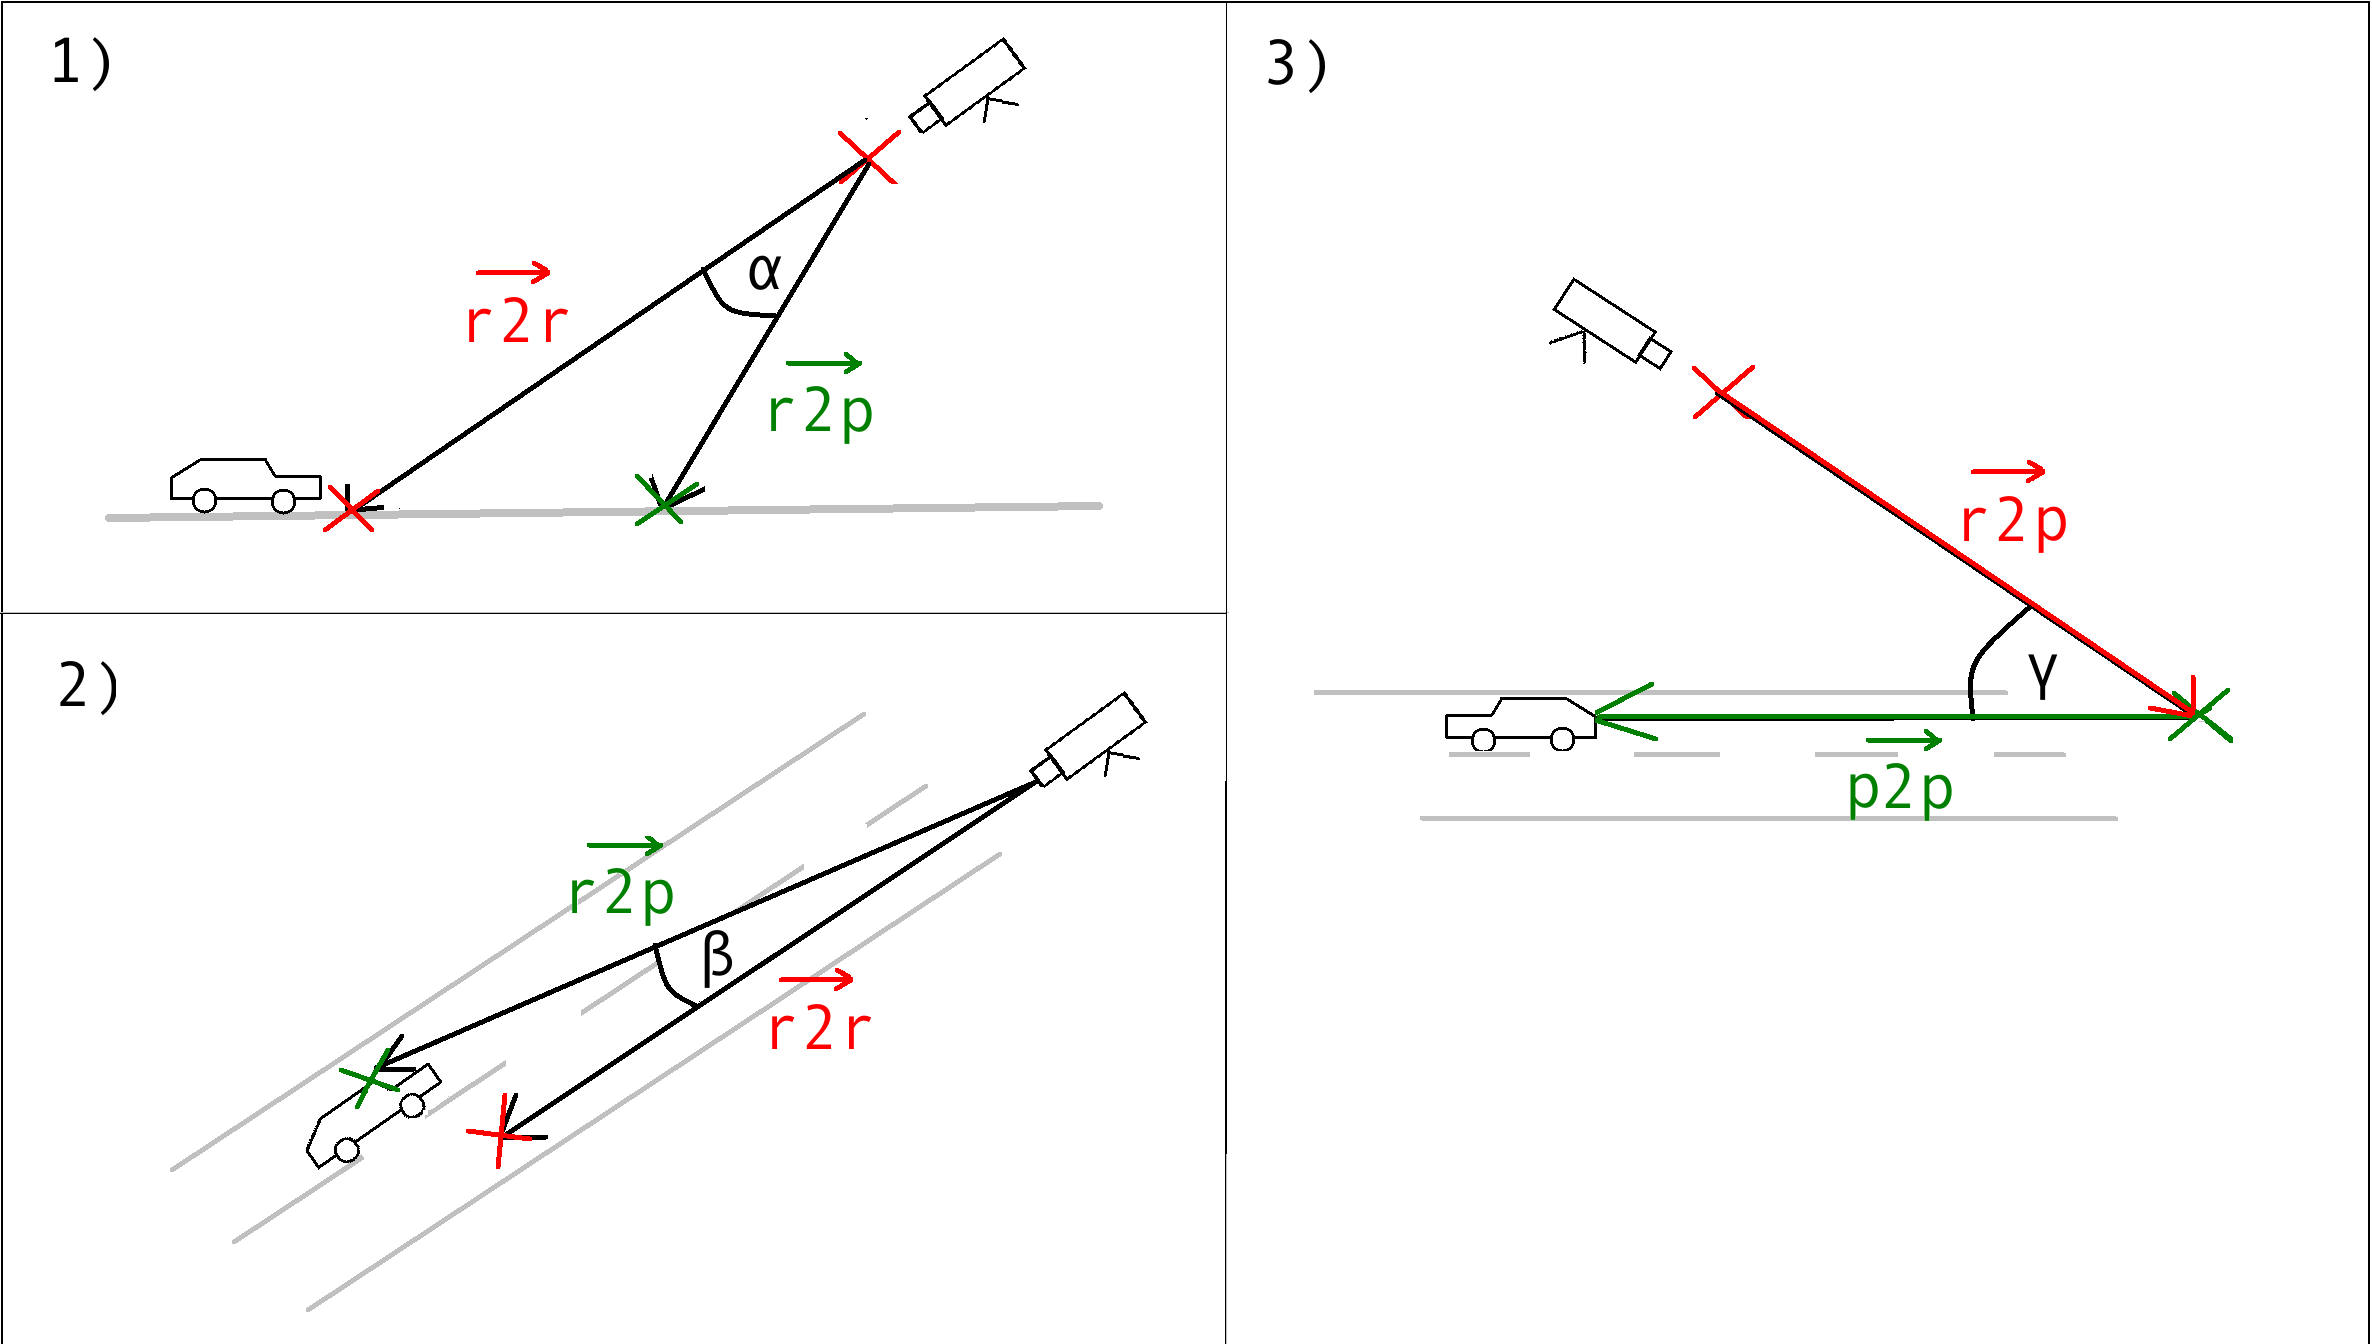
\includegraphics[width=1.0\textwidth]{obrazky-figures/radar_angles.png}
        \caption{Grafické znázornenie nami riešených a reprezenrtovaných uhlov. 1) Vertikálny 2) Horizontálny 3) Priestorový.}
        \label{fig:radar_angles}
    \end{figure}  

    \subsection{Vertikálny uhol}

      \hspace{0.6cm}Pomocou obrázku \ref{fig:radar_angles} časti 1) vidíme myšlienku pri získavaní hodnoty vertikálneho uhlu. Trojrozmerný priestor si premietnene do správneho dvojrozmerného pre získanie vertikálneho uhlu a to tak, že vynecháme jeho x-ovú zložku.
      Poznáme vektor radaru, teda bod v ktorom sa radar nachádza a bod na ktorý mieri, označme si ho ako $\overrightarrow{r2r}$(radar to radar).
      Rovnako poznáme aj aktuálnu pozíciu objektu. Teda vieme určiť vektor od umiestnenia radaru k aktuálnej pozícii objektu v priestore, označme si ho ako $\overrightarrow{r2p}$(radar to point).
      Ziskaný uhol medzi vektormi $\overrightarrow{r2r}$ a $\overrightarrow{r2p}$, je náš žiadúci vertikálny uhol. 

    \subsection{Horizontálny uhol}

      \hspace{0.6cm}Obdobne ako sme zíkali uhol vertikálny vieme získať aj uhol horizontálny, obrázok \ref{fig:radar_angles} časť 2). V tomto prípade pri premietnutí do dvojrozmerného priestoru vynecháme osu $z$, z troj rozmerného priesotoru.
      Rovnako využijeme vektory $\overrightarrow{r2r}$, $\overrightarrow{r2p}$ a získame požadovaný horizontálny uhol.
    \newline

  \subsection{Simulácia útlmu signálu}
    \hspace{0.6cm}Ďalej pracujeme s predstavou nášho priestoru, našej kocky, v ktorej je umiestnený náš radar so svojimi súradnicami rovnako ako aj jeho bod, ktorého pohyb pozoruje. Tieto dva bodi nám tvoria vektor, teda to ako radar mieri na fiktívnu cestu pod ním.

    Z jednej strany kocky na druhú stranu sa nám pohybuje náš objekt, v tomto prípade osobné vozidlo, ktoré je reprezentovaný zhlukom svojich bodov. Každý bod ma rovnakú rýchlosť v a smer pohybu, ktorý určuje jeho vektor pohybu. %Jedinečnú obsahuje len RCS charakteristiku.

    Náš radar imaginárne vysiela nepretržite v každom okamihu pohybu objektu paprsok, čo v našej simulácií znamená veľa výpočtov pre charakteristika tohto imaginárneho paprsku.
    \newline

    \subsection{Priestorový uhol}

    \hspace{0.6cm}Pre výpočet frekvencie signálu vracajucého sa do radaru budeme potrebovať priestorový uhol, ktorý zviera vektor radaru s vektorom pohybu objektu. Obrázok \ref{fig:radar_angles} časť 3).
    Vektor radaru je nám už dobre známy a máme ho označený ako $\overrightarrow{r2r}$. Vektor pohybu objektu nie je nič iné ako jeho aktuálna pozícia v priestore vo vzťahu s jeho pozíciou v priestore v dalšom časovom okamžiku, označme si ho $\overrightarrow{p2p}$ (point to point).
    Uhol, ktorý tieto 2 vektory zvierajú, je náš požadovaný priestorový uhol.

    \subsection{Vzdialenosť}

    \hspace{0.6cm}Vzdialenosť objektu od radaru je potrebné pre výpočet vracajúcej sa energie do radaru, ktorú získame z radarovej rovnice.
    V našom simulačnom prostredí pre získanie hodnoty vzdialenosti využijeme Euklidovu vzdialenosť, čo je metrika daná dvoma vektormi umiestnenými v priestore.
    V našom prípade vektora od bodu radaru k bodu objektu a vektora od bodu objektu k jeho smeru pohybu.

    \begin{figure}[h]
        \centering
        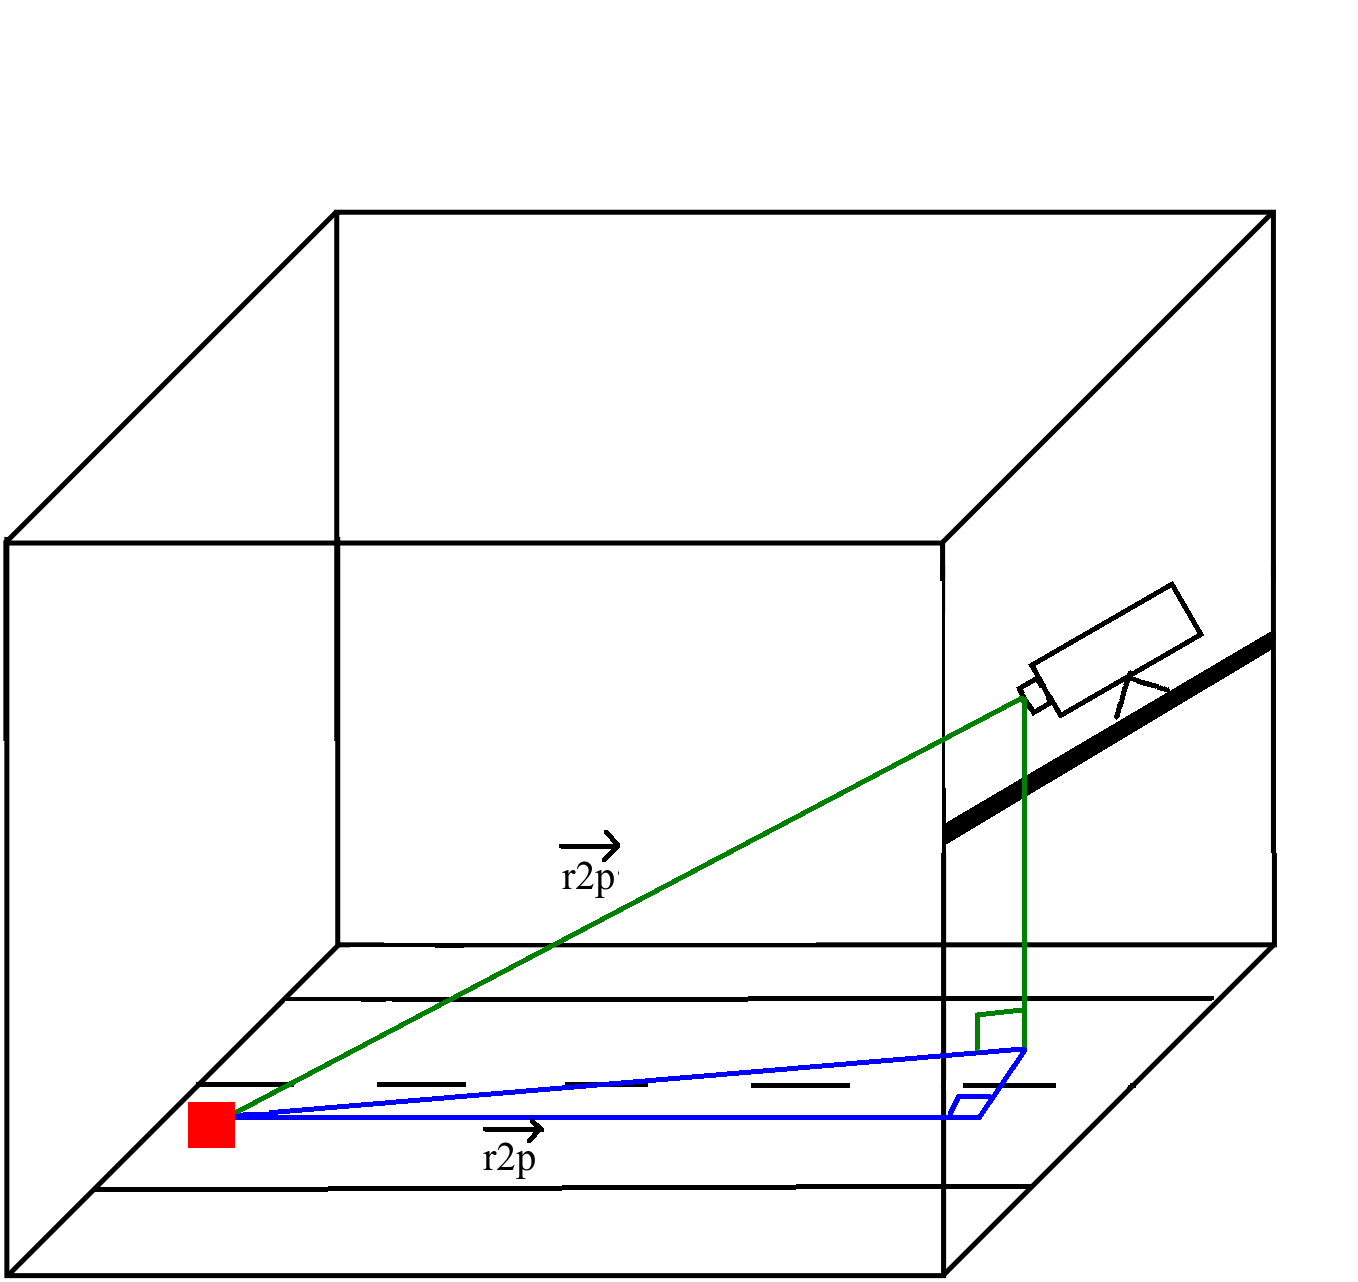
\includegraphics[width=0.5\textwidth]{obrazky-figures/euclid.png}
        \caption{Euklidova vzdialenosť.}
        \label{fig:euclid}
    \end{figure}      

    Euklidovu vzdialenosť teda vypočítame ako absolútnu hodnotu normály pozície radaru od ktorej odčítame pozíciu objektu.


    \subsection{Prijatý signál}

    \hspace{0.6cm}Po správnom získaní priestorového uhlu, ktorý zviera vektor radaru s verktorom pohybu objektu, sme schopný v každom okamžiku pohybu objektu získať veľkosť sígnalu vracajucého sa od objekt späť do radaru a to pomocou vzťahu:

      \begin{equation} %\label{eq:0}
        F_{r} = 2 * v * \frac{F_{t}}{c} * cos(\gamma)
      \end{equation}   

    Kde rýchlosť objektu $v$ je nami dopredu určená, rovnako ako aj vysielacia frekvencie antény $Ft$ v podiely s rýchlosťou svetla $c$. To všetko je v súčine s kosínusom náško priestorového uhlu $\gamma$.
    Celý tento vzťah nie je nič iné ako aplikácie dopplerovho javu.

    \subsection{Radarová rovnica}

    \hspace{0.6cm}Pre náš finálny výpočet a to kalkuláciu energie, ktorá sa po odraze od objektu do radaru vráti musíme aplikovať nami upravenú radarovú rovnicu, ktorá bola  kompletné vysvetlená v teoreticek časti \ref{radarovarovnica}.

      \begin{equation} %\label{eq:0}
        %P_{r} = \frac{P_{t} * F_{r} * F_{t} * RCS}{(4\pi)^{2} * d^{4} * loss}
        P_{r} = \frac{\lambda * RCS * \sqrt[10]{10^{loss}}}{(4\pi)^{2} * d^{4}}
      \end{equation}   

      \begin{equation} %\label{eq:0}
        \lambda = \frac{c}{F_{t}}
      \end{equation}         

      Hodnota $P_{r}$ predstavuje výkon prijatého signálu, ktorý touto rovnicou získame. Vlnová dlžka ($\lambda$) je podiel rýchlosti svetla $c$ s hodnotou frekvencie akú mal vyslaný signál $F_{t}$ z radaru, rovnica \ref{eq:55}. Veličina $RCS$ nám je dobre známa ako Radar cross-section. Hodnota $loss$ predstavuje stratu signálu získanú výpočtami uhlov z charakteristiky antény, na ktorú sme aplikovali logaritmus.
    %$(4\pi)^{2}$
      Hodnota $d$ je vzdialenosť radaru od objektu. Kedže je vysielač aj príjmač umiestnený na spoločnej anténe, umocníme to na štvrtú.


\chapter{Implementácia}
  \hspace{0.6cm}Táto kapitola sa venuje samotnému prevedeniu návrhu do prostredia programovacieho prostredia Matlab, čo môžeme považovať za cieľ tejto bakalárskej práce. V tejto implementácii sme použili nástroje Matlab, Gimp a Excel. Prvý spomenutý nástroj bol použitý s licenciou poskytnutou Ústavom počítačovej grafiky a multimédií, Fakulty Informačných Technológií, Vysokého učení technického v Brne. Zvyšné dva spomenuté nástroje boli použité s opensource licenciou.

  Pre overenie informácií z algoritmov spracovania signálov, ktoré sme získali z použitých zdojov a rovnako aj pre nové kalkulácie bude využité matematické prostredie Matlab. To bolo zvolené pretože obsahuje veľa vstavaných funkcií, ktoré nám zjednodušia prácu.  

  Radar KMC-4, ktorý sme sa rozhodli pre túto simuláciu používať ako referenčný má svoje vlastnosti, ktoré musíme implementovať aj do našeho simuláčného radaru. Všetky tieto údaje boli predom získane vyrobcom tohto radaru, firmou RFbeam a sú umiestnené v jeho datasheete \cite{kmc4sheet}, preto ich nemusíme nadobudnúť experimantálne.

  \begin{itemize}
    \item Vysielacia frekvencia radaru KMC-4 je 24.150GHz
    \item Zisk antény je 13dB
    \item Zisk vysielača
    \item Zisk príjmača
  \end{itemize}  

  \section{Charakteristika antény}
    Hardwarový modul samotného radaru mieri na určitý bod. Nemôže vysielať a príjmať všetky svoje paprsky do všetkých bodov a smerov rovnomerne. Charakteristika antény, resp. anténový diagram reprezentuje aké je potlačenie vysielaného signálu v decibeloch, jednotlivo v horizontálnom a vertikálnom smere vzhľadom na vysielaní signálu od vektoru radaru v uhlových stupňoch. Tento údaj je obsiahnutý v datasheete a je len graficky znázornený.

    \begin{figure}[h]
        \centering
        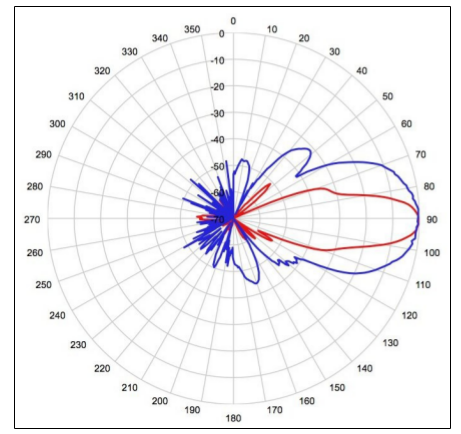
\includegraphics[width=.7\textwidth]{obrazky-figures/kmc4_antenna_char.png}
        \caption{Diagram graficky zobrazujúci charakteristiku antény. Ktorý sme použili ako zdroj pre našu textovú verziu charakteristiky antény.\cite{kmc4sheet}.}
        \label{fig:kmc4_antenna_char}
    \end{figure}

    Preto je potrebné extrahovať tento útlm antény pre každý stupeň jednotlivo. Pre tento prípad sme použili jednoduchú metódu za pomoci programu Gimp a jeho nástroja pre zmeranie uhlu a to nasledovne. Umiestnili sme jeden koniec pravítka do stredu obrázku a druhý koniec po čiare doprava vedúcej k uhlu 90 stupňov. Tento nástroj ďalej fungoval ako uhlomer a s uhlom v strede obrázku sme pohodlne vyčitali pre každý červený (horizontálny) a modrý (vertikálny) bod jeho útlm v určitom uhle \ref{fig:kmc4_antenna_char}.

    Celý tento proces sa zapisoval do súboru vo formáte .csv. Jeden súbor obsahuje informácie v rozsahu $0^{\circ}-180^{\circ}$, delených po jednom stupni. Pre vertikálny smer a druhý súbor v rovnakom rozsahu pre horizontálny smer.

    180 získaných hodnôt pre nás avšak nebude dostačných. Nato aby sme signál rekenštruovali musíme dodržat Nyquistov teorém a predpokladaná frekvencia simulácie bude 10 kH. To nám spôsobí, že nami získané hodnoty su vo veľmi malom rozsahu a výsledný graf by bol zkockovatelý. Preto musíme tieto hodnoty interpolovať.

    Pôvodný interval hodnôt obsahuje $180$ bodov, ten vynásobime tísickou a pre týchto $180 000$ bodov sa malý interval interpoluje do veľkého pomocou matematickej metódy spline. To znamená, že pre väčší internal sme našli približné hodnoty funkcie medzi bodmi v danom menšom intervaly.

    %Na spracovanie útlmu bola vytvorená pomocna funkcia matlabu anntenna\_system\_diagram.m. Ktorej vstupné hodnoty sú vstupný uhol pre ktorý chceme zistiť útlm a orientácia aby sme vedeli či chceme vrátiť útlm v horizontálnom alebo vertikálnom smere. Táto funkcia vo svojom tele pomocou informácie o orientácií načíta potrebný .csv súbor, ktorý prechadza a v ňom nájde požadovaný uhol pre ktorý vráti jedinú hodnotu a to útlm v dB.

    Nami získaný a spracovaný útlm potrebuje pre využitie správny uhol, pre ktorý sa bude určovať. Ten musíme získat v našom trojrozmernom priestore jednotlivo pre horizontálnu a vertikálnu zložku dvojrozmerného priestoru.

    Vertikálny a Horizontálny uhol, ktorý sme výpočtami získali teraz vieme v každom okamžiku simulácie získať uhol radaru voči objektu. Tento uhol použijeme v nami predom pripravených .csv dátach a tým a získame stratu signálu v dB, osobitne pre horizontálny a vertikálny smer v danom časovom okamžiku a usporiadaní objektov priestore. Následne tieto 2 hodnoty vertikálneho a horizontálneho smeru medzi sebou vynásobíme a dostaneme aktuálnu stratu signálu v dB, pre náš bod v priestore voči radaru v danom časovom okamžiku. 
  

  \section{Simulácia modelovanej scény}
    \hspace{0.6cm}Samotná simulácia je tvorená spojeným všetkých menších celkov, ktoré boli doposiaľ v častiach Návrhu a Implementácie vysvetlnené.

    Celá simulácia sa odvíja od počtu simulačných krokov, ktoré učujú ako podrobne bude každý pohyb objektu spracovaný. Čím viac simulačných krokov, tým podrobnejšie dáta získame, teda tým podrobnejší výsledok zobrazíme. Optimálny počet simulačných krokov našej simmulácie bude $10 000$. Čo bude vo vzťahu s 10kH, ktorá je odporúčaná frekvencia simulácie pre splnenie Nyquistovho teorému. V prípade menšieho počtu krokov by mohlo dôjsť k antializasingu.\newline

    \textbf{Vstup simulácie}

    Program získava vstupné dáta zo súboru input.json, ktorý obshauje stromovú štruktúru vstupných dát vo formáte JSON (JavaScript Object Notation).
    Tento spôsob bol zovelný z dôvodu možného ďalšieho využitia tohto simulátora výzkumnou skupinov, bez toho aby museli mať hlbšie povedomie o podrobnom funkčnosti kódu, resp. zasahovať priamo do neho.
    Všetky potrebné a modifikovateľné premenné sa dajú pohodlne a prehľadne upravovať pomocou tohto jazyka. Ktorý poskytuje možnosť jednoduchého a zrozumiteľného organizovania dát do polí, alebo agregovania do objektov. Je nezávislý na platforme.
    Týmto spôsobom dokážeme oddeliť zdrojový kód Matlabu od užívateľa. Teda vstup programu môže elegantne ovládať pomocou vstupného súboru a nemusí zasahovať priamo do matlabového zdrojového súboru.
    Samotný matlab, ho môže jednoducho a elegantne načítať pomocou pomocnej kninžnice JSONLab.

    Vstupné dáta sú reprezentované v minimálne dvoch súboroch. V prvom scene.json, je definované ako bude vyzerať scéna a jej všetky nastavenia. Z globálnych nastavení obsahuje všetky informácie o radare, jeho vysielaciu frekvenzcie a zisk antény. Z nastavení simulácie obsahuje počet krokov aký simulácia vykoná a prepínače pomocou ktorých si je užívateľ schopný nastaviť či mu ma simulácie počas celého behu zobrazovať ako sa priestor mení, reps. či mu to ma zobraziť len na začiatku pre kontrolu. 
    Ďalej si z nastavení scény môže uživateľ nastaviť veľkost scény v akej chce simulovať, pozíciu radaru v priestore a pozíciu miesta kam radar miery.

    Druhý vstupný súbor reprezentuje nastavenie modelu. Pre každý model sa odporúča vytvoriť vlastný súbor. Ten obsahuje informácie o postavení modelu v priestore, jeho rýchlosti a hodnote RCS.\newline

    \textbf{Vizualizácia vstupu}

    Kedže samotný beh programu je výpočetne náročný, predtým ako ho užívateľ spustí je rozumné, aby si overil ako jeho vstupné dáta vyzerajú. To znamená aby videl ako bude objekt v prostredí reprezentovaný, aký bude vektor jeho pohybu a v akých pozíciach sa bude náchadzať. Zapnutie tohto testovacieho rozhrania môže jednoducho pomocou nastavenia $global$ a jeho prepínača $Test_simulation_setup$ na hodnotu $on$.
    Matlab mu pomocou jednoduchého plotu zobrazí prostredie spolu so všetkými bodm, ktoré reprezentujú užívateľom zadané objekty.
    Vzhľadom na plánované dalšie využitie tohto programu to hodnotím ako potrebnú časť programu.\newline

    \textbf{Spracovanie bodov}

    V programe Matlab sa simulácia bodov v našom navrhnutom prostredí vytvára, rovnako ako aj riadi pomocou nástroja HGtransform, ktorý je implicitne obsiahnutý v prostredí Matlab. Tento nástroj spravuje všetky body priestoru, ktoré sme mu vytvorili. S bodmi, ktoré sú na to vopred určené pohybuje v smere v aký sme mu predom definovali. Predpokladáme a určuje pohybu ako homogenný jav, teda náš pohybujúci objekt nebude zrýchľovat ani spomaľovať.

    V našom trojrozmenrom prostredí nimi môže pohybovať až vo všetkých troch osiach. Nám pre simuláciu vozidla na vozovke bude stačiť práve jeden až maximálne dva. V budúcnosti pri simulácii objektov pohybujúcich sa vzduchom by sa mohli zísť aj tretia osa.\newline    

    \textbf{Jadro}

    Jadro simulácie tvorí cyklus, ktorý vykonáva presný počet iterácií, ktorý sa rovná počtu simulačných krokov. V každej jednej iterácii sa pre každý pohybujúci bod jednotlivo urči jeho nová aktuálna pozícia, pričom poznáme aj jeho pozíciu v dalšej iterácií. Tu získame jednoducho tým, že k aktuálnej pozícii pripočítame posun v priestore aký mu určí funkcia HGtransform. 

    Pre statické body, ako pozíciu radaru v priestore, či bod na ktorý v priestore mieri nám stačí získat práve raz.
    \newline

    Po získani potrebných pozícií bodov v pristore pre daný okamžik, prebiehajú všetky potrebné výpočty a to:
    \begin{itemize} 
      \item získavanie vzdialenosti
      \item výpočet horizontálneho a vertikálneho uhlov
      \item Čo vyústi k výpočtu strát signálu
    \end{itemize}

    Po získaní týchto potrebných medzivýpočtov ich náslende použijeme v rovniciach pre:

    \begin{itemize}
      \item výpočet rozdielu signálu odpovedajúceho Dopplerovej frekvencii $F_{r}$ v $Hz$
      \item výpočet výkonu prijatého signálu vo W pomocou radarovej rovnice $P_{r}$
    \end{itemize}

    Výsledkom tohto celého procesu iterácií bude dvojrozmerné pole, ktoré bude obsahovať hodnotu výkonu prijatého signálu. Pre každý jeden bod v jeho každom časovom okamžiku.\newline

    \textbf{Generovanie signálu}

    Po skončení tohto sledu iterácií a získaní všetkých potrebných dát a ich naplnení do finálneho poľa výsledkov sa spustí ešte jeden identický cyklus s rovnakým počtom iterácií, ktory generuje počiatočný signál v ktorom sa zakompunuje náša prijatá frekvencia $F_{r}$ spolu s výkonom prijatého signálu $P_{r}$.\newline  

    \begin{equation} \label{eq:631}
      \varphi_{d_{t}} = 2\pi * F_{r} * d_{t}
    \end{equation}

    \begin{equation} \label{eq:632}
      result(n) = sqrt(P_{r})*e^{j(\varphi_{1} + \varphi_{d_{t}})}
    \end{equation}

    \begin{equation} \label{eq:633}
    \varphi_{1} = \varphi_{1} +  \varphi_{d_{t}}
    \end{equation}        

    \textbf{Spojenie bodov objektu}

    Doposiaľ boli body reprezentujúce objekt, ktorý radar sleduju spracovávané samostatne, cez všetky doteraz vysvetlnené kroky.
    V tejto časti spracovania signálu sa tieto body zlúčia dohromady a to tak spôsobom, že ich hodnoty v každom bode spočítame dohromady.
    Teda pre každú žložku signálu v danom bode a danom časovom okamžiku vznikne jedna v danom časovom okmažiku, ktorá bude súčet hodnôt všetkých bodov v danom časovom okamihu.\newline

    \textbf{Spracovanie signálu}

    V poslednej fáze spracovania signálu nám ostáva už len tento signál segmentovať pomocou Hammingoveho okna cez ktoré tento signal rozdelí na menšie, lepšie spracovateľné časti - rámce.Dĺžka rácma je vypočítaná pomocou primernej hodnoty signálu v danom intervaly, cez funkciu $mean$.

    Tieto rámce ďalej spracuje Rýchla Fourierova transormácia o čo sa postará funkcia matlabu $fftshift$.

    \begin{lstlisting}
        seg = seg - mean(seg);
        X = fftshift(fft(seg.*hamming(SEG_LEN)', FFT_LEN));
    \end{lstlisting}

    
  \section{Reprezentácia dát}
  \hspace{0.6cm}Po získaní dát pre všetky naše body pohybujúceho sa objektu sa tieto body medzi sebou dohromady sčítajú, čím vytvoria jeden bod, ktorý reprezentuje vlastnosti všetkých ako jeden objekt. Ten je následne rezprezentovaný jednorozmerným poľom hodnôt, ktorého veľkosť je priamo úmerná počtu simulačných krokov. Každý tento prvok obsahuje svoju reálnu a imaginárnu zložku.\newline

  Dáta sa najlepšie a najnázornejšie reprezentujú pomocou grafu a teda funkcie |plot| rozhrania matlab. Samostatne vykresľujeme graf pre reaálnu a imaginárnu zložku, resp. rozlíšime tieto dve zložky rôznymi farbami.

\chapter{Testovanie a výsledky}

  Výsledkom celého procesu simulácie signálu, od vstupný dát, až po kompletné výpočty, ktoré sme si doposiaľ v tejto práci spomenuli je súbor hodnôt, ktoré obsahujú reálnu a imaginárnu zložku signálu.
  To považujeme za finálny výstup tohto programu. Pre názorne a lepšie pochopenie výsledku tieto hodnoty zobrazíme v podobe grafu reprezentujúceho časové spektrum oproti frekvencii. Kde môžme vidieť amplitúdy reprezentujúce narušenie signálu, čo je spôsobéne objektom, ktorý popred radarom prešiel.
  Ešte lepšiu reprezentácia týchto dát je možné vidieť na spektograme priamo pod grafom. 
  Dôležité je si uvedomiť, že signál ma najväčšiu amplitúda prave tam, kde je imaginárna zložka čísla v nule, teda fáza signálu sa pretínu s nulou.

  Tento finálny výsledok môže byť ďalej spracovaný algoritmami výzkumnej skupiny.

  Porovnanie s realnymi dátami.

  Výstupom simulátoru je surový signál odpovedajúci Dopplerovským posunom vznikajúcim v namodelovanom prostredí.  

\chapter{Záver}

  \section{Zhodnotenie výsledkov}
    \hspace{0.6cm}

  \section{Dalšie pokračovanie práce}
    \hspace{0.6cm}Po dôkladno získavaní informácií a naštudovaní problému sa bude táto práce ďalej uberať v praktickom smere. Pomocou získaných algoritmov a informácií sa pokusím implementovať program pre šírenie radarových vĺn vo vnútri modelovanej scény, najprv v programe Matlab a tak vo forme knižnice C++.

    Po úspechu tejto časti modelovania, budem pokračovať simulačnými experimentov kde sa budú porovnávať reálne a simulované dáta. Vzhľadom na tieto výsledky sa bude ladiť mnou vytvorený model. 

    Vo výsledku by mala táto práca znázorňovat ako sa širia elektormagnetické vlny priestorom v porovnaní s reálnym radarom \ref{fig:kmc4_odchylka}.



%=========================================================================